%++++++++++++++++++++++++++++++++++++++++
% Don't modify this section unless you know what you're doing!
\documentclass[letterpaper,12pt]{article}
\usepackage[utf8]{inputenc}
\usepackage{float}
\usepackage{tabularx} % extra features for tabular environment
\usepackage{amsmath}  % improve math presentation
\usepackage{graphicx} % takes care of graphic including machinery
\usepackage[margin=1in,letterpaper]{geometry} % decreases margins
\usepackage{cite} % takes care of citations
\usepackage[final]{hyperref} % adds hyper links inside the generated pdf file
\usepackage[table,xcdraw]{xcolor}
\hypersetup{
	colorlinks=true,       % false: boxed links; true: colored links
	linkcolor=blue,        % color of internal links
	citecolor=blue,        % color of links to bibliography
	filecolor=magenta,     % color of file links
	urlcolor=blue         
}
%++++++++++++++++++++++++++++++++++++++++


\begin{document}

\title{Práctica 2 - Ruteo}
\author{Matthew Aguerreberry, Natasha Tomattis}
\date{\today}
\maketitle

% \begin{abstract} 
% \end{abstract}


\section{Practica de Ruteo - RIP}
\begin{figure}[ht] 
        
	\centering 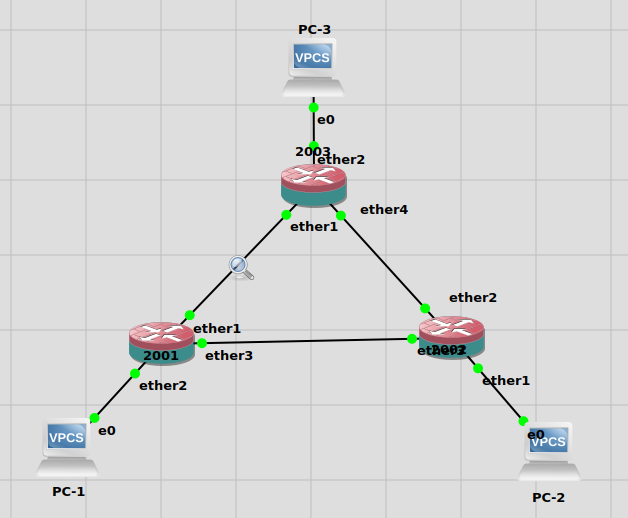
\includegraphics[width=0.8\columnwidth]{figure/topo.png}
	%\includegraphics[width=1.0\columnwidth]{sr_setup.pdf}
	\caption{
			\label{fig:samplesetup} % spaces are big no-no 
			Implementación Ejercicio 1.
	}
\end{figure}
	\begin{enumerate}
		\item \textbf{¿RIPv1 es un protocolo de vector-distancia o estado-enlace? ¿Y RIPv2? ¿Conoce algún otro protocolo de ruteo de la misma familia?} \\
		Por su comportamiento y la forma de determinar la ruta mas corta tanto RIPv1 como RIPv2 son de tipo vector-distancia. El protocolo de ruteo Enhanced Interior Gateway Routing Protocol (EIGRP) pertenece a la misma familia de RIP, es un protocolo propietario de Cisco el cual fue convertido a código abierto en 2013.
		\item \textbf{¿Pertenecen al grupo de IGP o EGP?}\\
		RIP pertenece al grupo de IGP (\textit{Internal Gateway Protocol}, o protocolos de ruteo interno)
		\item \textbf{¿Qué mejoras incluye RIPv2 con respecto a RIPv1?}\\
		Por un lado RIPv2 permite la distribución de actualizaciones a través multicast (usando el grupo fijo 224.0.0.9), a diferencia de RIPv1 que utiliza direcciones broadcast. Por otro lado, RIPv1 solo soporta esquemas de direccionamiento IP classful, ya que en su cabecera no admite el agregado de mascaras de subred, RIPv2 amplia su cabecera y permite de esta forma esquemas de direcciones IP classless. Además, RIPv2 agrega autenticación entre los peers.
		\item \textbf{¿Cuál es el valor máximo de hop-count permitido en RIP? ¿Qué significa la métrica 16?}\\
		El valor máximo de hop-count es de 15. La métrica 16 indica que la ruta es inalcanzable.
		\item \textbf{ ¿Qué son los timers: update, invalid y flush?}\\
		\textit{Update}: Define cada cuanto tiempo se deben enviar actualizaciones a un vecino. El valor predeterminado es de 30 segundos.\\
		\textit{Invalid}: Por defecto es de 180 segundos y corresponde al tiempo en el cual una ruta se almacenará en la tabla de enrutamiento hasta que se considere inválida.\\
		\textit{Flush}: Define el tiempo que toma el router en eliminar una ruta desde que se declaró como inválida. Por defecto son 240 segundos.
		\item \textbf{¿Cómo funcionan Triggered Updates, Counting to infinity,Split-Horizon y Poisoned Reversed?}\\
		\textit{Counting to infinity}: Es una inconsistencia que surge ya que los routers propagan lentamente los mensajes de actualización de una ruta que no es mas alcanzable.  Ya que la ruta queda en loop y la distancia a esa ruta se empieza a incrementar debido a que, por ejemplo,  
		dos routers vecinos se podrían enviar infinitamente una ruta. Por esta razón se establece una cantidad máxima de 16 saltos en las rutas.\\
		\textit{Triggered Updates}: Es un mecanismo que fuerza al router a enviar inmediatamente una actualización ante un cambio en las tablas de ruteo.\\
		\textit{Split-Horizon}: Impide que se envíen actualizaciones de ruta por la interfaz por la que se aprendió dicha ruta.\\
		\textit{Poisoned Reversed}: Cuando a un router se le cae una ruta, él debe mandar una actualización con métrica 16 para declarar la ruta como \textit{unreachable}.

		\item \textbf{Conectar los routers según el diagrama de la figura 1.}
		\item \textbf{Configurar las interfaces de acuerdo al diagrama.}
		\item \textbf{Configurar RIPv1 en todas las interfaces. ¿Es posible alcanzar todas las redes?} \\
		Depende de las redes que se distribuyan por RIP. 
		
		\item \textbf{Realice una captura entre los routers 2001 y 2003:}
		\begin{itemize}
			\item \textbf{¿Qué protocolo y puerto de capa de transporte utiliza para funcionar?} \\
			UDP puerto 520.
			\item \textbf{¿Qué tipos de mensajes RIP se intercambian entre esos routers?} \\
			RIP response.
			\item \textbf{¿Se realiza algún tipo de sincronización entre los procesos RIP de los routers antes de intercambiar algún tipo de información?} \\
			No.
			\item \textbf{¿Por qué intercambian ciertas redes con métrica 16 si las redes están activas?} \\
			Al estar activado el mecanismo de Split-Horizon las rutas aprendidas por dicha interfaz son declaradas como inalcanzables.
		\end{itemize}
		
		\item \textbf{Modificar el direccionamiento de la siguiente manera: cambiar la mascara de las redes 192.168.x.0/24 a /26}
		\item \textbf{¿Es posible alcanzar todas las redes? ¿Por que?} \\
		El comportamiento no se modifica porque siguen siendo subredes classful distintas.
		\item \textbf{Modifique  el  direccionamiento  de  la  red  entre  2002  y  VPCS-2  a  la dirección 192.168.10.64/26. ¿Que sucede con el ruteo?} \\
		Se genera conflicto ya que la subred entre 2001 y VPCS-1 equivale a la misma subred classful.
		\item \textbf{¿Como lo solucionaría? Encuentre los comandos para solucionar este problema sin cambiar el direccionamiento} \\
		Configurando las interfaces en RIPv2 que admite direccionamiento classless.
		\item \textbf{Realice nuevamente una captura entre los routers 2001 y 2003;}
		\begin{itemize}
			\item \textbf{¿Se modifican el protocolo y capa de transporte que utiliza RIPv2 con respecto a RIPv1?} \\
			No.
			\item \textbf{¿Se modifica el formato del paquete RIP con respecto a la anterior versión? ¿Se agregan nuevos campos?} \\
			Si, se agrega los campos \textit{Netmask, Next Hop, Route Tag}.
			\item \textbf{¿Qué información agrega para que cada router aprenda correctamente las demás redes?} \\
			La máscara de subred.
		\end{itemize}
		\item \textbf{Si por algún motivo RIP deja de funcionar en uno de los routers, ¿Qué pasaría en la red? Por ej., suponga que se cae RIP en router 2001.} \\
		En los routers 2003 y 2002 se va a vencer el timer invalid de la ruta hacia la red 192.168.10.0/24 volviéndola inalcanzable. 
		\item \textbf{¿Qué es la distancia administrativa? ¿Para qué se utiliza? ¿Es lo mismo que la métrica?} \\
		La distancia administrativa indica la fiabilidad de un protocolo de enrutamiento, depende de cada fabricante. Se utiliza para determinar una ruta cuando hay dos o más rutas a un mismo destino para dos protocolos de enrutamiento. \\
		La métrica se utiliza para comparar rutas al mismo destino pero del mismo protocolo de enrutamiento.
		\item \textbf{Active ruteo estático en todo los routers de manera que  se puedan alcanzar todas las redes pero que sirvan como rutas de backup (RIP debe tener prioridad)}
		\begin{figure}[ht] 
        
			\centering 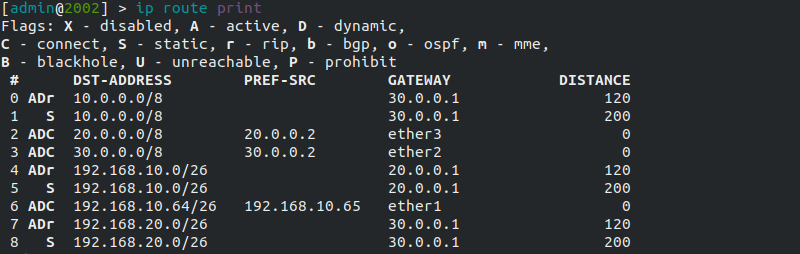
\includegraphics[width=0.8\columnwidth]{figure/static.png}
			\caption{
					\label{fig:samplesetup} % spaces are big no-no 
					Ruteo estatico activado en router 2001.
			}
		\end{figure}
		\item \textbf{¿Usaría RIP como protocolo de ruteo en una red de tamaño mediano o grande?} \\
		RIP presenta desventajas en redes de mayor escala debido a la cantidad de mensajes de actualización que se generarían periódicamente y el tiempo de convergencia es muy lento. Además, al distribuir muchas redes el tamaño de los paquetes de actualización se vuelve considerablemente grande. 
	\end{enumerate}
	\subsection{Enlaces consultados}
	\begin{itemize}
		\item{HCNA Networking Study Guide}  \\
		\textit{Springer. Huawei Technologies Co., Ltd.},Ch 8.2 RIP.
		\item{Temporizadores de RIP}  \\
		\url{http://www.redescisco.net/sitio/2010/07/19/temporizadores-de-rip/}
	\end{itemize}
	\end{document}